\documentclass[letterpaper,english, 12pt]{scrreprt}
\usepackage[T1]{fontenc}
\usepackage{array}
\usepackage{graphicx}
\usepackage{float}
%\usepackage{titlepic}
\newcolumntype{C}[1]{>{\centering\let\newline\\\arraybackslash\hspace{0pt}}m{#1}}

\title{Musical Heart Rate Adjuster}
\subtitle{Software Engineering Project \\ https://github.com/revansopher/HeartRateAdjuster}
\author{Group \#12}
%\titlepic{
\includegraphics{img/title.png}}

\begin{document}
\maketitle

\tableofcontents

\section*{Team Profile}
\begin{description}
	\item[Nikhil Shenoy] C++, Python
	\item[Revan Sopher] Android programming, web programming, Java, Python
	\item[Tae-Min Kim] Java, C++, Python
	\item[Samani Gikandi] Java, C, Ruby, Network programming, Device driver/firmware programming
	\item[Kenny Bambridge] IOS programming, web programming, Java, Python
	\item[Jonathan Chang] documentation, organization, C++
\end{description}
 
\chapter{Customer Statement of Requirements/Project Proposal}
 
\section{Problem}
There seems to be a growing concern over the bevy of health-related issues that society faces: cancer, obesity, heart diseases. This is evidenced by the estimated \$25.9 billion that consumers spent on fitness membership in 2013 or the government's seemingly carte blanche spending on "perfecting" the healthcare.gov website. While it is impossible to completely eliminate health problems, we focus on a small, albeit interesting subset of the health industry - personal health monitoring. Just like "an apple a day keeps the doctor away," our project seeks to maintain the personal health of an individual, keeping him in the best physical shape possible, and reducing the risk of health problems.
 
\subsection{More Specifically}
Lack of education about proper fitness is a widespread problem. Many people in the country would like to exercise and stay in shape, but only a small subset of those people know how to monitor their health in a way that allows them to stay fit. There are several methods out there which people can use to get the proper information; tools such as fitness blogs, the President's Council on Fitness, Sports, and Nutrition, and the classic visit to the doctor's office are all excellent examples. However, many people don't know about those methods or choose not to utilize them, and they do their body a disservice by performing exercises that could be detrimental to their health. The Internet is littered with articles such as "9 Exercises You're Doing Wrong" and "The 7 Fitness Myths You Need to Know". With information like this readily available to exercisers, it can be hard to find correct information. And even if one does find correct information, he must check to see if that information applies to a person with his body shape and size. The general problem of finding correct exercise information is that there is no set standard; there is no "one size fits all" set of guidelines which one can follow to have an effective workout. Everybody's body responds differently to different exercises, so the best that the medical community can do is to provide a set of recommendations for people of the most average body type. While this set of recommendations is good in the general, they will never tailor to the needs of one's body and workout. Finding the correct exercise information for one's body type is quite a difficult problem, and it will continue to be a problem until a solution is provided to track each person's exercise routine.
 
Of all the different metrics for measuring the quality of one's fitness, heart rate is the most important factor in determining whether a workout was effective. Monitoring one's heart rate is useful because it determines whether the exerciser is performing his exercise safely as well as successfully. Experts recommend that one's target heart rate during exercise should be between 60-85\% percent of the maximum heart rate, and that anything higher than 85\% increases cardiovascular and orthopedic risk to the exerciser. Naturally, the target heart rate varies for people of different ages, so one should always take this into account before starting a fitness regimen. Also, the frequency of exercise before the new regimen should be considered. If one has not exercised frequently before starting the new regimen, then he should start exercising at a rate that is towards the lower end of the target heart rate zone and then gradually increase his activity once his body gets accustomed to the exercise. Heart rate is a significant, if not the most important, factor in determining whether a workout was done correctly and effectively, and it must be monitored closely in order to prevent injury.
 
Unfortunately, there are people who don't know how to correctly monitor their heart rate, and they mistakenly create a certain fitness plan based on wrong information and end up not optimizing their workout. They go to the gym, run on the treadmill at a light pace, and consider that enough to maintain their health. They do not check their heart rate and make sure they are in the safe region of activity. This critical lack of measurement affects the entire workout. For an exercise to be effective, one must maintain a heart rate that is within the target range for an extended period of time. If not, the exerciser either puts himself at risk of injury or completes a workout that does very little to improve his fitness. Some use exhaustion and soreness after a workout as a judge of an effective workout. Although these methods do give an indication as to how effective the exercise was, they do not provide an insightful and accurate description of one's health. As a result, these people continue bad habits and routines that hinder their progress to stay fit; in fact, they may not be even making progress.
 
A solution to the problem of uninformed exercise must have three main components; it must include all relevant medical data such as heart rate information, create a fitness plan that fits relatively well to the client's body, and provide the client with feedback about the effectiveness of his workout. Once all these components come together, the client will be able to correctly monitor his health during exercise and get the most out of his workout.
 
\subsection{Background}
A healthy lifestyle depends upon a plethora of factors including environment, nutrition, socialization, and mental stability. However, we identified physical fitness and sleep as the two key factors to leading a healthy lifestyle. Their importance cannot be overstated.
 
Physical fitness or exercise fortifies the body, allowing one to stay in shape, avoid injuries, develop confidence, become stronger, and sleep better. Sufficient physical activity can reduce the risk of such symptoms as stress, depression, diabetes, high blood pressure, osteoporosis, and obesity.
 
Meanwhile, sleep is critical to the mind. It refreshes the brain, helps with daily functioning, uplifts one's mood and emotional well being, increases productivity, and improves learning and memory. "Good" sleep can lower the probability of contracting the following: heart disease, kidney disease, high blood pressure, diabetes, and stroke.
 
\subsection{Devices and Specifications}
Motoactv:\\
600 MHz ARMv7 CPU\\
256MB RAM\\
8GB Flash Memory\\
802.11B/G/N\\
Bluetooth 4.0 low energy\\
ANT+ for connectivity to fitness sensors\\
1.6" 220x176 LCD\\
\\
Heart Rate monitor:\\
Either ANT+ or Bluetooth to connect to Motoactv and/or smart phone\\

Our project is centered around the Motoactv device, whose specifications are listed above.The Motoactv is essentially a Motorola-manufactured smartwatch that combines features that would normally be found on a GPS, pedometer, and music player. It also runs Android, contains bluetooth, and provides web-based analytics. We plan on using the Motoactv in conjunction with a compatible heart rate monitor because we are primarily interested with the ability of our music to affect heart rate. Besides monitoring the subject's heart rate and collecting the relevant data, the Motoactv will also be responsible for running our customized Android music player as well as hold our special music library. We wish to to categorize how strenuous the user's current workout is, and encourage them to select a more challenging category to push themselves. Our music player will then play a song and adjust its tempo based on the selected category and the measured heart rate.

Zeo:
The Zeo headband, similar to a personal EEG, uses conductive sensors to collect electrical signals produced by the brain, as wella s eye movement. Then, Zeo takes this information and produces graphs to summarize the user's sleep, pointing out trends or critical points such as the ranges of REM sleep. It also offers a "Sleep Score." (We may use the Zeo to analyze and compare the quality of sleep when our Musical Heart Rate Adjuster is being used. More research will be done on the product and its features when we receive the device.)
			 
\section{Solution}
It has been well documented that exercise and sleep both hold a significant impact on heart rate. However from experience, we believe that the link between exercise and sleep and heart rate holds true for the converse as well. One of the targets of a good workout is an increased heart rate. On the other hand, high-quality sleep entails a decreasing heart rate.
			 
Our proposed solution is designed to affect people's health by providing limited control to their heart rates. Our Musical Heart Rate Adjuster is targeted to operate in two areas where it can be the most effective - workouts and sleep - which in turn offer the aforementioned health benefits. We do not plan on adjusting heart rate with the intent of skipping the rigors of exercise or the process of falling asleep; on the contrary, we wish to adjust heart rate to induce better quality workouts and sleep.
			 
Our plan is composed of a few steps. First, we intend to increase the effectiveness of workouts by matching heart rate to an appropriate selection and tempo of music. This music can be adjusted accordingly to stimulate heart rates to reach a desired intensity of exercise. The music, which will be discussed later, performs the task of simulating workout difficulty. As an added benefit, studies have shown exercising while listening to music to provide many benefits, such as increased motivation and endurance, distraction from otherwise unbearable stress, and increased heart rate, among others.
			 
Then, we seek to improve the quality of sleep by finding soothing music to gradually slow down a user's heart rate. In this instance, we use music as an instrument to aid users in falling asleep more quickly, and hopefully improve the performance of their rest. This will be determined by the sleep graphs provided by the Zeo Sleep Monitor. Looking at the peaks and troughs of the graph will allow us to recognize when the user has fallen asleep, as well as the time and quality of his deepest slumber. Listening to right music can also improve the quality of sleep; for instance, music by classical composer Mozart has been shown to increase health factors such as relaxation and mental stimulation.
			 
\subsection{Music}
We utilize music to affect heart rate in two ways. In addition to identifying and playing music with speeds in the same vicinity as heartbeat, we also wish to be able to adjust the tempo of the music. A simple compound microscope has both a coarse adjustment knob as well as a fine adjustment knob. Our song library will organize songs into different categories, acting as a coarse adjuster for heart rates. Meanwhile, to add a little fine-tuning to adjust the heart rates, we will either write or find an existing application for an audio tempo changer. Given current heart rate, and subsequently, current music tempo, we will continually adjust the music tempo while measuring for changes in heart rate. This will occur until we hit the specified target heart rate, give or a take a few BPM. Thus, if there is no difference in heart rate, either the targeted heart rate has been reached - otherwise,  the music tempo has not been adjusted enough.
			 
We are interested in analyzing the magnitude of the effect of our music application on heart rate and finding a rough correlation based on the data that the Motoactv provides. All parties should remember, however, that correlation is not causation. While we take the assumption that the general public will react to music in similar ways (music with a slower tempo will decrease heart rate while music with a higher tempo will increase heart rate), it is difficult to know how every individual will react to the same music and can never be 100 percent accurate.

This will probably take some experimentation with test subjects in several situations such as rest, running, weight-lifting, and playing basketball. Time-permitting, we will also find the ability of music to slow down heart rate and affect sleep by analyzing the Zeo sleep monitor graphs. As a side experiment, we could measure the effect of several well-known classical songs on sleep quality.
			 
Finally, we will be able to develop an algorithm for ranking the songs that induce the best performance. Even better, we could potentially toy around with machine learning to have our algorithm improve after more and more data sets. With the application of machine learning, each user's individual MotoActv device may correct itself in the case that a specific user does not follow the general trend as stated previously (a user's heart rate might increase from slow music rather than fast music). This way, our Motoactv will be able to increase both exercise and sleep performance through our own custom music player application, located on and loaded by the device. This application will utilize the user's music library stored locally on the device's memory.

\subsection{Web Platform/Database}
Users will want to monitor their personal health status, so our project will include a web component. The Motoactv device does have its own website, but our project is primarily interested with music and heart rate, so we will be able to better customize our own website, tailoring it to a potential customer's needs in this context. The Zeo device has limited support because the company went out of business, so we will need our own website to combine information from both the Motoactv and the Zeo. Data from the Motoactv and the Zeo will go to a web server, which will then go to a database performs storage and processing. Our website will pull information from the database and display a useful graph of the correlation between music and heart rate. (The exact features of this website will be determined later on because it is one of the later steps of our project. A diagram will also be provided later.)

\subsection{Product Usage}
\begin{itemize}
	\item The heart rate monitor should only be worn while it is in use - while sleeping or while exercising. While it is safe to wear the heart rate monitor during other times, there will be no benefit unless the application is currently running. 
	\item Users may choose to use the Musical Heart Rate Adjuster while not sleeping or exercising if they wish to adjust their heart rate for alternate reasons (possibly for playing video games or preparing for an exam). 
	\item The user will run the android application, and then input a target heart rate. The software will then choose a song based on your current heart rate and begin to either raise or lower it. Once the target heart rate is obtained within a certain tolerance, the software will work to maintain this heart rate rather than increasing/decreasing it.
	\item Music will be selected from the user's own personal music library (which should be stored on the flash memory of the MOTOACTV) to either increase or decrease the user's heart-rate. Music will be played by our software.
	\item The software will select and play music according to the user's current heart rate in real-time as it receives information from the connected heart rate monitor.
	\item Music will be delivered through the headphone jack on the MOTOACTV or through any bluetooth device.
	\item Receive information on the songs that are listened to in relation to their usage of the MOTOACTV. (What songs were listened to, which songs were the most effective at changing their heart rate, etc.)
\end{itemize}

\subsection{Product Ownership (tentative)}
Our team will be divided into three smaller sub-teams of two individuals each, the pairings listed below. Each sub-team will be responsible for music, hardware, or web and provide a brief description of their work on a shared Google drive folder. They will also include the necessary UML diagrams and charts. Every week (or bi-week) we will meet together for 1-3 hours during the timeframe determined by When2meet. During the meeting, we will have a specific agenda that primarily involves the week's progress and upcoming deliverable. Our discussion will probably be centered along the following questions: 1) What did you work on this past week? 2) What do you plan on working on next week? 3) Are there any changes that need to be made to the project? Every week, a different team member will take the lead for the next deliverable to ensure that everything is on time.          	

\begin{itemize}
	\item Nikhil and Samani will develop a system to select or modify a track based on requested BPM. If possible they will incorporate machine learning into the system.
	\item Jonathan and Kenny will design the website converts data into useful graphs for users to view and evaluate. They will also work on a database that receives, stores, and processes the data from the Motoactv, before sending it to the website.
	\item Revan and Tae-min will program the Android application and work on interfacing with the heart rate monitor.
\end{itemize}

\section{Glossary of Terms}
\begin{description}
	\item[Electroencephalography (EEG)] EEG is the study of oscillations of brain electrical potentials which are recorded from the human scalp. EEG measures voltage fluctuations which result from ionic current flowing within neurons inside of the brain. This will be achieved via our Zeo sleep monitor.
	\item[Electrocardiography (ECG)] ECG is an interpretation of the electrical activity of the heart over a period of time as measured across the thorax or chest. This interpretation is produced by attaching electrodes to the surface of the skin. This is generally used to measure the heart’s electrical conduction system by picking up electrical impulses generated by the polarization and depolarization of cardiac tissue.

	\item[Beats per Minute (BPM)] BPM is the amount of times that the heart beats given one minute of time.

	\item[Resting Heart Rate] The resting heart rate is the heart rate measured while the subject is both awake and inactive, not having performed physical activity prior. This resting heart rate, measured in bpm, is the initial value that the user should have before using our device to raise or lower their heart rate.

	\item[Database] Databases are a place to store information. In our case, this is where we will store and process important data received from our health devices, allowing our website to simply act as a pleasant interface for the user.

	\item[Target Heart Rate] The target heart rate is the heart rate which the user wishes to achieve. This will be lower than the recorded resting heart rate if the user is attempting to sleep, and higher than the recorded resting heart rate if the user is planning to work out. The user's maximum heart rate is based on how old the user is (220 minus the user's age), and the recommended target heart rate while exercising is between 50 and 85 percent, depending on how active the user normally is. While sleeping, people's heart rates generally drop approximately 8 percent from their resting heart rate, so the user's target heart rate should be approximately [(heart rate before sleeping)*0.92]

	\item[Smartphone] Smartphones are mobile phones which contain features that are more advanced than basic mobile phones. In our case, any Android device which has the capability to use Bluetooth will suffice to interact with the sensors which will be put on the body.

	\item[Heart Rate Monitor] A device which is able to monitor the user’s heart rate. In our experiment we will be using a third party heart rate monitor (worn as a chest strap) which has sensors that are connected to the skin along with the MOTOACTV watch. The chest strap will record the heart rate while the watch will display the user’s current heart rate in real time.
\end{description}

\chapter{System Requirements}
Based upon our consumer needs, we derived a list of requirements for our system to
possess. For features that must be implemented by the system, we state that "The
user shall," whereas for features that are preferred, but not "mandatory," we state
that "The user should." For each requirement, we assign an identifier in the form of
REQ-x, as well as a priority weight from 1 to 5. A higher priority weight indicates
that the corresponding requirement is more essential to the success of the project,
and more critical to fulfilling the customer's needs.

\section{Functional Requirements}
\begin{center}
	\begin{tabular}{|C{2cm}|C{2cm}|C{8cm}|}
		\hline
			Identifier & Priority & Description\\
		\hline
			REQ-1 & 5 &  The system shall log user BPM data using the Heart Rate Monitor sensor.\\
		\hline
			REQ-2 & 5 & The system shall sync the information to Android device via Bluetooth.\\
		\hline
			REQ-3 & 4 & The system shall allow user to select a target heart rate on the Android application.\\
		\hline
			REQ-4 & 3 & The system shall determine a song from the user’s music library in the tempo range of the user’s selection.\\
		\hline
			REQ-5 & 5 & The system shall play the designated song through either headphones or Bluetooth speakers to adjust user heart rate.\\
		\hline
			REQ-6 & 3 & The system shall store the BPM data in the database.\\
		\hline
			REQ-7 & 2 & The system shall output useful graphs of user workout data on the website to demonstrate the effects of music on BPM.\\
		\hline
			REQ-8 & 1 & The system should adjust the tempo of the song to further match the user’s BPM and stop when within a defined range.\\
		\hline
			REQ-9 & 1 & The system should allow the user some control when they use the website. That is, they should be able to customize the look and feel of the account on their website as well as the details of how the data is displayed (type of graph or specific categories of data).\\
		\hline
			REQ-10 & 1 & The system should rank the songs that induce the best performance and use machine learning to improve the song selection algorithm.\\
		\hline
                        REQ-11 & 1 & The user should be able to change the current song if he is unsatisfied with it. \\
                \hline
                        REQ-12 & 1 & The user should be able to view his current heart rate as long as the chest strap is recording that information. \\
		\hline
	\end{tabular}
\end{center}

Our functional requirements spell out the behavior of our system and reaction to
user input. Our system is composed of several aspects such as the heart rate
monitor, android device, server and database, and website. These requirements
describe some of the interactions between these components and the effects that
he system as a whole produces. The images in the appearance requirements section
ater on provide more insight on the requirements and functionality of our system.

\section{Non-Functional Requirements}
\begin{center}
	\begin{tabular}{|C{2cm}|C{2cm}|C{8cm}|}
		\hline
			Requirement & Priority Weight & Description \\
		\hline
			REQ-1 & 5 & The Android interface shall have a minimal number of navigation menus; the user should not need more than three taps to find the information he needs \\
		\hline
			REQ-2 & 5 & The user shall not be able to directly modify any data in the database. All data must be programmatically gathered and processed \\
		\hline
			REQ-3 & 4 & The user shall use his same credentials for login on the mobile application as he will use for the website \\
		\hline
			REQ-4 & 3 & The web interface shall have a minimal, but sufficient number of options to display different information about the user's workout. \\
		\hline
			REQ-5 & 3 & The user should wear the device only when the user wishes to alter their heart-rate; the device will not provide useful information if it is worn when the user does not plan to increase or decrease their heart-rate. \\
		\hline	
			REQ-6 & 3 & Both the web site and the Android application should be intuitive and simple to use. \\
		\hline
	\end{tabular}
\end{center}

Meanwhile, our non-functional requirements are more descriptive than practical,
listing the qualities of our system. These requirements are based on the term
FURPS+, which includes functionality, usability, reliability, and performance.

\section{On-Screen Appearance Requirements}
This diagram highlights our system architecture: Our heart rate monitor senses the
user’s BPM and transmits the data to the Android phone via Bluetooth as requested
by the app. The phone then wirelessly uploads the data to the server and database
which processes the data. The phone app is then able to select the appropriate
songs, and the website is able to display suitable graphs.

\begin{figure}[H]
	\centering
	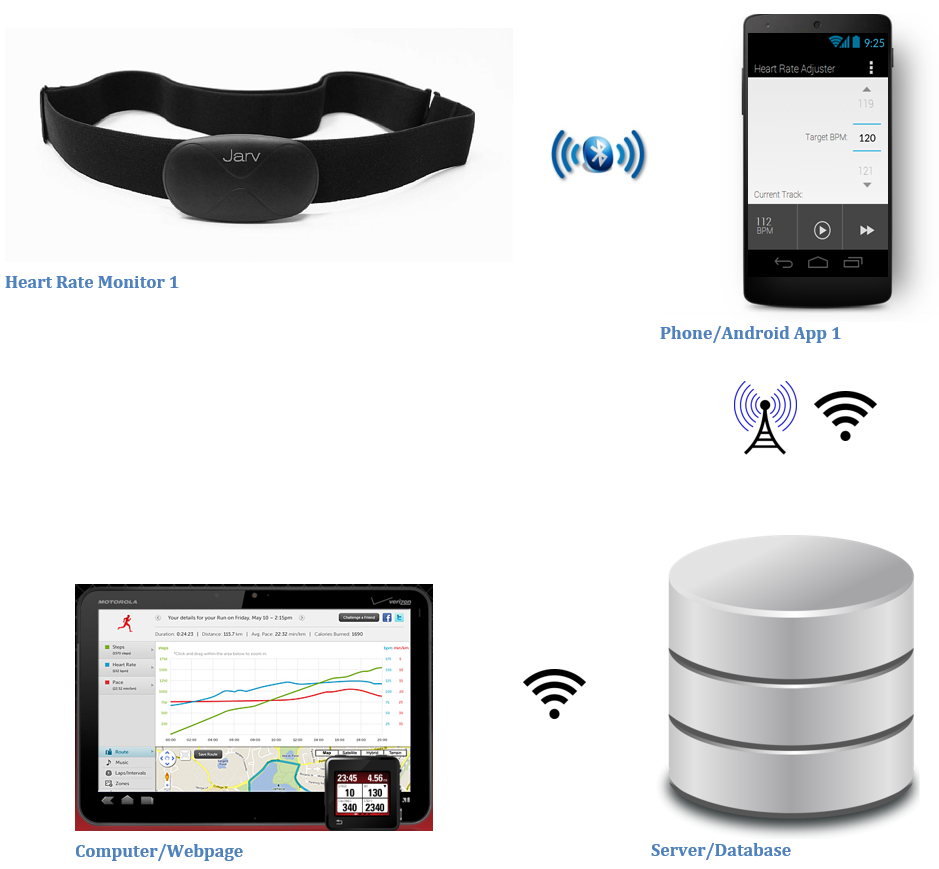
\includegraphics{img/system.png}\\
	\caption{System design}
\end{figure}

\subsection{Mobile Application}

\begin{figure}[H]
	\centering
	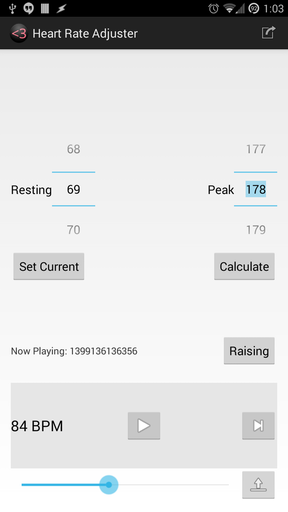
\includegraphics{img/mobile_ui/1.png}\\
	\caption{The main screen of the app provides a menu button, selectors for Target Peak and Resting BPM, a display of the current track, a display of the current BPM, and the option to Play/Pause and Skip the current track.}
\end{figure}

\begin{figure}[H]
	\centering
	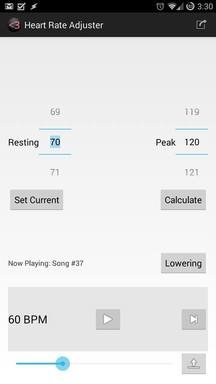
\includegraphics{img/mobile_ui/2.png}\\
	\caption{Pressing the ``Raise/Lower'' button toggles between attempting to raise or lower the BPM.}
\end{figure}

\begin{figure}[H]
	\centering
	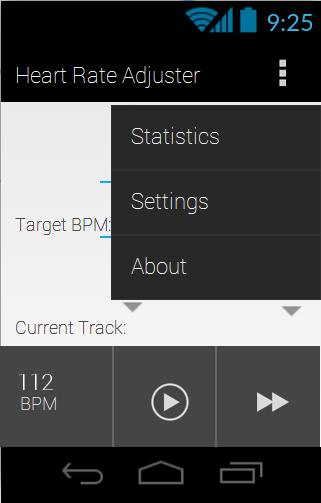
\includegraphics{img/mobile_ui/3.png}\\
	\caption{Pressing the menu button opens the context menu, providing the option to edit settings and view information about the app.}
\end{figure}

\begin{figure}[H]
	\centering
	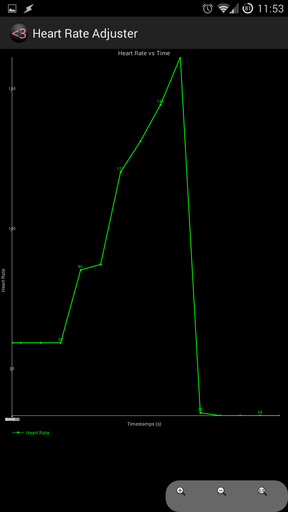
\includegraphics{img/mobile_ui/4.png}\\
	\caption{The settings page allows the user to open a menu to Log in, to edit the location of the media library (this is done via the OS's directory selection), and configure additional parameters such as music generation (if there is time to implement this feature).}
\end{figure}

\begin{figure}[H]
	\centering
	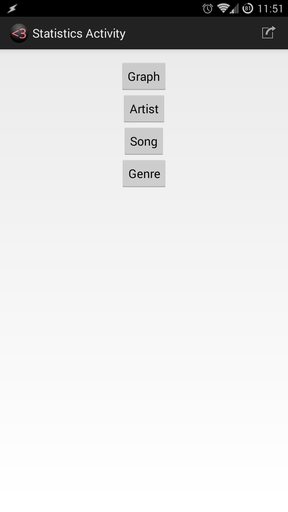
\includegraphics{img/mobile_ui/5.png}\\
	\caption{Selecting the Log in option prompts the user for their credentials.}
\end{figure}

\begin{figure}[H]
	\centering
	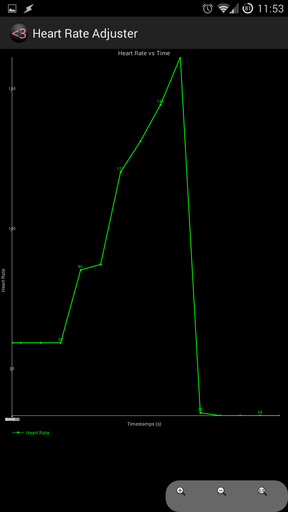
\includegraphics{img/mobile_ui/6.png}\\
	\caption{Selecting the About option from the context menu provides a description of the application.}
\end{figure}

\subsection{Stakeholders}
Stakeholders include individuals and organizations which are interested in the completion and use of a given product. The amount of stakeholders and different types of stakeholders relies on the versatility and ease-of-use of the product in question. Due to this software’s very simple interface and design, stakeholders may include users of all ages and multiple types of organizations who are interested in obtaining easier sleep or a more energetic workout. Examples of potential stakeholders include:
\begin{enumerate}
	\item Individuals who are interested in maintaining their health personally without outside help. With the many functions of the application, users have the capability of maintaining their health without the need to consult other people. People who are introverts or do not have easy access to another person who is able to easily analyze the individual’s personal health would be very interested in this application. After running this application through their workout or sleep, users can easily consult the graphs which are produced rather than consulting a personal trainer or doctor about their health.
	\item Organizations that specialize in helping people fall asleep. Rather than having to prescribe pills to every customer who has trouble sleeping, they will have the option to suggest this product to the customer for minor cases. While prescribing pills may tend to have slightly more dangerous side-effects, our product does not introduce any chemicals to the body which may potentially cause harm to the consumer. Organizations who are interested in a cleaner alternative to help people with their sleeping problems would be stakeholders for this product.
	\item Organizations that specialize in promoting exercise and personal health. Not only does this product help those who are trying to sleep, but also those who wish to be more fit. While personal trainers may know how to help the customers and be great motivators, organizations may be interested in helping a larger pool of customers without having to increase the amount of hands that they have working. With this product organizations may grant customers the option of being self-sufficient, helping to increase self-esteem, as well as a great motivator as the application works to increase the user’s heart rate allowing them to push onward and burn calories easily.
	\item Organizations interested in monitoring and researching people’s health. While there are many users who are able to use the product’s graphs and understand how their health and workout are, there are many users who still prefer the assistance of outside sources. This product may also be used by these outside sources to help them collect extra data on an individual’s health. Rather than having the customer come to their location and run a couple tests in a single day, the organization will have the ability to provide this product to the customer and collect more regular data to understand the customer’s day-to-day life rather than a couple of tests run at their office.
\end{enumerate}

More specifically, this product may see stakeholders in:
\begin{itemize}
	\item Personal Trainers
	\item Athletes
	\item Coaches
	\item Doctors
	\item Researchers
	\item Pharmacies
	\item Therapists
	\item General population
\end{itemize}

\subsection{Actors and Goals}
Actors can be defined as are people or devices that will directly interact with the product, and can also be loosely labeled as either “initiators” or “participators”. These actors will have a specific goal with the given product, which is what the actors are attempting to achieve by interacting with the system. Actors and their respective goals are:
\begin{center}
	\begin{tabular}{|l|l|}
		\hline
		\emph{Actor} & \emph{Actor's Goal} \\\hline
		User(initiator)& To increase heart rate for exercising\\\hline
		User(initiator)& To decrease heart rate for sleeping\\\hline
		User(initiator)& To analyze health information from given graphs\\\hline
		Chest strap (participator)& To monitor the user's heart rate\\\hline
	\end{tabular}
\end{center}
This product is one which only requires the interaction of one human actor, the user of the product. While there is the potential for other humans to interact with the user’s health information which is produced, only the user himself is considered an actor. The headband and chest strap are participating actors that are worn by the user to monitor information and relay the information via Bluetooth back to the smartphone which is running the application.

\section{Use Cases}
Use Cases are specific tasks that are created together by the designer and the client to simulate what the client wants out of his software solution. They are meant to describe the main features of the project such that the designer can easily address the needs of the client and create a product around those needs. Below is a casual description of the use cases for the reader to get a general idea of how the software should be used. Later, fully described use cases are shown for additional insight into the different cases.

\subsection{Casual Description of Use Cases}
\begin{center}
        \begin{tabular}{|C{2cm}|C{2cm}|C{10cm}|}
                \hline
                        Use Case & Action & Description \\
                \hline
                        UC-1 & increaseHeartRate & The user should enter a target heart rate and begin the workout \\
                \hline
                        UC-2 & decreaseHeartRate & The system will bring the user's heart rate down from an exercise rate to a resting rate \\
                \hline
                        UC-3 & getNextSong & The user can elect to change the song if he does not like the current one. The new song will be adjusted to reflect the current heart rate of the user and keep the user on track towards the target heart rate. \\
                \hline
                        UC-4 & pausePlayback & The user can pause the playback of the music if he would like. \\
                \hline
                        UC-5 & getStatistics & The user can request the statistics about the current workout. This can be performed while the workout is in progress or after the workout has been completed. \\
                \hline
                        UC-6 & getHeartRate & The user can view his current heart rate. This can be used when the user does not want to see all of the statistics from the workout and just wants his heart rate. \\
                \hline
        \end{tabular}
\end{center}

\subsection{Detailed Description of Use Cases}

\begin{center}
        \begin{tabular}{|C{15cm}|}
                \hline
                        \textbf{Use Case UC-1: increaseHeartRate}\\
                \hline
                        \begin{flushleft}
                                \textbf{Related Requirements: } REQ-1, REQ-3, REQ-4, REQ-5, REQ-6, REQ-8
                        \end{flushleft}
                        \begin{flushleft}
                                \textbf{Initiating Actor: } User
                        \end{flushleft}
                        \begin{flushleft}
                                \textbf{Actor's Goal: } To enter a target heart rate and begin the workout
                        \end{flushleft}
                        \begin{flushleft}
                                \textbf{Preconditions: }
                        \end{flushleft}
                                \begin{itemize}
                                        \item The system displays the selection menu for heart rate
                                        \item The user is exercising at a heart rate which is below the peak rate
                                \end{itemize}
                        \begin{flushleft}
                                \textbf{Postconditions: }
                        \end{flushleft}
                                \begin{itemize}
                                        \item The system starts recording the heart rate of the user and the data from the workout if not already recording.
                                        \item The system uses the recorded heart rate to run the music selection algorithm
                                \end{itemize}
                        \begin{flushleft}
                                \textbf{Flow of Events for Main Success Scenario: }
                        \end{flushleft}
                                \begin{itemize}
                                        \item $\rightarrow$ User enters the target heart rate into the application.
                                        \item $\leftarrow$ System initates a five-second countdown until the start of the exercise.
                                        \item User begins his workout
                                        \item $\leftarrow$ System uses music algorithm to play appropriate music.
                                        \item $\leftarrow$ System begins recording data about the workout and stores it in the database.
                                \end{itemize}
                %\hline
        \end{tabular}
\end{center}

\begin{center}
        \begin{tabular}{|C{15cm}|}
                \hline
                        \textbf{Use Case UC-2: decreaseHeartRate}\\
                \hline
                        \begin{flushleft}
                                \textbf{Related Requirements: } REQ-1, REQ-3, REQ-4, REQ-5, REQ-6, REQ-8
                        \end{flushleft}
                        \begin{flushleft}
                                \textbf{Initiating Actor: } User
                        \end{flushleft}
                        \begin{flushleft}
                                \textbf{Actor's Goal: } Reach a resting heart rate
                        \end{flushleft}
                        \begin{flushleft}
                                \textbf{Preconditions: }
                        \end{flushleft}
                                \begin{itemize}
                                        \item The user is exercising at a heart rate which is above that of the resting rate.
                                \end{itemize}
                        \begin{flushleft}
                                \textbf{Postconditions: }
                        \end{flushleft}
                                \begin{itemize}
                                        \item The system starts recording the heart rate of the user and the data from the workout if not already recording.
                                        \item The system uses the initial resting heart rate as a target for the music selection algorithm
                                        \item The user is returned to the resting heart rate he was at before the workout.
                                \end{itemize}
                        \begin{flushleft}
                                \textbf{Flow of Events for Main Success Scenario: }
                        \end{flushleft}
                                \begin{itemize}
                                        \item $\rightarrow$ User selects "Lower" option on main UI.
                                        \item System feeds previous resting heart rate as a target for the music selection algorithm. Initiates the decline.
                                        \item $\leftarrow$ System initiates a five-second crossfade as the music algorithm starts playing slower music.
                                        \item User starts walking to the tempo of the music to cool down.
                                        \item $\leftarrow$ System uses music algorithm to play appropriate music. Records the current heart rate to manage the decline of the heart rate.
                                \end{itemize}
                %\hline
        \end{tabular}
\end{center}

\begin{center}
        \begin{tabular}{|C{15cm}|}
                \hline
                        \textbf{Use Case UC-3: getNextSong}\\
                \hline
                        \begin{flushleft}
                                \textbf{Related Requirements: } REQ-5, REQ-8, REQ-11
                        \end{flushleft}
                        \begin{flushleft}
                                \textbf{Initiating Actor: } User
                        \end{flushleft}
                        \begin{flushleft}
                                \textbf{Actor's Goal: } To play a different song
                        \end{flushleft}
                        \begin{flushleft}
                                \textbf{Preconditions: }
                        \end{flushleft}
                                \begin{itemize}
                                        \item The user is unsatisfied with the song currently being played
                                \end{itemize}
                        \begin{flushleft}
                                \textbf{Postconditions: }
                        \end{flushleft}
                                \begin{itemize}
                                        \item A different song is being played at the same rate at which the previous song was playing
                                \end{itemize}
                        \begin{flushleft}
                                \textbf{Flow of Events for Main Success Scenario: }
                        \end{flushleft}
                                \begin{itemize}
                                        \item $\rightarrow$ User selects the "Next Song" button.
                                        \item System retrieves next track from recommendation algorithm.
                                        \item $\leftarrow$ System begins playing next track
                                \end{itemize}
                %\hline
        \end{tabular}
\end{center}

\begin{center}
        \begin{tabular}{|C{15cm}|}
                \hline
                        \textbf{Use Case UC-4: pausePlayback}\\
                \hline
                        \begin{flushleft}
                                \textbf{Related Requirements: } REQ-1, REQ-5
                        \end{flushleft}
                        \begin{flushleft}
                                \textbf{Initiating Actor: } User
                        \end{flushleft}
                        \begin{flushleft}
                                \textbf{Actor's Goal: } Pause the playback of music
                        \end{flushleft}
                        \begin{flushleft}
                                \textbf{Preconditions: }
                        \end{flushleft}
                                \begin{itemize}
                                        \item The system is playing music
                                \end{itemize}
                        \begin{flushleft}
                                \textbf{Postconditions: }
                        \end{flushleft}
                                \begin{itemize}
                                        \item The system stops recording the heart rate of the user and the data from the workout.
                                \end{itemize}
                        \begin{flushleft}
                                \textbf{Flow of Events for Main Success Scenario: }
                        \end{flushleft}
                                \begin{itemize}
                                        \item $\rightarrow$ User selects "Pause" option on main UI.
                                        \item $\leftarrow$ System stops playing music.
                                \end{itemize}
                %\hline
        \end{tabular}
\end{center}

\begin{center}
        \begin{tabular}{|C{15cm}|}
                \hline
                        \textbf{Use Case UC-5: getStatistics}\\
                \hline
                        \begin{flushleft}
                                \textbf{Related Requirements: } REQ-6, REQ-7, REQ-10
                        \end{flushleft}
                        \begin{flushleft}
                                \textbf{Initiating Actor: } User
                        \end{flushleft}
                        \begin{flushleft}
                                \textbf{Actor's Goal: } Return statistics about the user's workout.
                        \end{flushleft}
                        \begin{flushleft}
                                \textbf{Preconditions: }
                        \end{flushleft}
                                \begin{itemize}
                                        \item The user has finished his workout and would like to see his statistics
                                        \item The user also has the option to display the statistics during the workout
                                \end{itemize}
                        \begin{flushleft}
                                \textbf{Postconditions: }
                        \end{flushleft}
                                \begin{itemize}
                                        \item The Android application displays the graphs of the user's heart rate versus time, along with other metrics.
                                \end{itemize}
                        \begin{flushleft}
                                \textbf{Flow of Events for Main Success Scenario: }
                        \end{flushleft}
                                \begin{itemize}
                                        \item $\rightarrow$ User selects the "Display Statistics" option.
                                        \item System retrieves data from the current workout and creates graphs of the various metrics.
                                        \item $\leftarrow$ System displays the graphs to the user.
                                \end{itemize}
                %\hline
        \end{tabular}
\end{center}

\begin{center}
        \begin{tabular}{|C{15cm}|}
                \hline
                        \textbf{Use Case UC-6: getHeartRate}\\
                \hline
                        \begin{flushleft}
                                \textbf{Related Requirements: } REQ-12
                        \end{flushleft}
                        \begin{flushleft}
                                \textbf{Initiating Actor: } User
                        \end{flushleft}
                        \begin{flushleft}
                                \textbf{Actor's Goal: } View the current heart rate.
                        \end{flushleft}
                        \begin{flushleft}
                                \textbf{Preconditions: }
                        \end{flushleft}
                                \begin{itemize}
                                        \item The device should already be monitoring the user's heart rate.
                                \end{itemize}
                        \begin{flushleft}
                                \textbf{Postconditions: }
                        \end{flushleft}
                                \begin{itemize}
                                        \item The current heart rate is displayed on the screen of the Android application.
                                \end{itemize}
                        \begin{flushleft}
                                \textbf{Flow of Events for Main Success Scenario: }
                        \end{flushleft}
                                \begin{itemize}
                                        \item $\rightarrow$ User selects the "Display Heart Rate" option.
                                        \item System retrieves current heart rate from chest strap.
                                        \item $\leftarrow$ System displays the heart rate to the user.
                                \end{itemize}
                %\hline
        \end{tabular}
\end{center}


\chapter*{Individual Contributions Breakdown}
\begin{center}
	\begin{tabular}{|l|C{2cm}|C{1.5cm}|C{1.5cm}|C{1.5cm}|C{1.5cm}|C{1.5cm}|}
		\hline
								&Kenny Bambridge&Jonathan Chang	&Samani Gikandi	&Tae-Min Kim&Nikhil Shenoy	&Revan Sopher\\ \hline
			Problem Statement	&		X		&		X		&		X		&		X	&		X		&		X\\ \hline
			Glossary of Terms	&				&				&				&		X	&				&		\\ \hline
			System Requirements	&				&		X		&				&			&		X		&		\\ \hline
			Func. Requirements	&				&		X		&				&			&				&		\\ \hline
			Non-Func. Req.		&				&				&				&			&		X		&		\\ \hline
			Appearance Req.		&		X		&		X		&				&			&				&		X\\ \hline
			Project Management	&				&		X		&				&			&		X		&		X\\ \hline
	\end{tabular}
\end{center}

\chapter*{References}

References 1-5 are the final project reports of the previous groups who worked on the Personal Health Monitoring projects. They were consulted in conjunction with Professor Marsic's Software Engineering textbook as a guide for formatting guidelines, content ideas, and inspiration. 
\begin{verbatim}
[0] http://www.ece.rutgers.edu/~marsic/books/SE/book-SE_marsic.pdf
[1] http://www.ece.rutgers.edu/~marsic/books/SE/projects/HealthMonitor/2013-g7-report3.pdf
[2] http://www.ece.rutgers.edu/~marsic/books/SE/projects/HealthMonitor/2013-g8-report3.pdf
[3] http://www.ece.rutgers.edu/~marsic/books/SE/projects/HealthMonitor/2012-g1-report3.pdf
[4] http://www.ece.rutgers.edu/~marsic/books/SE/projects/HealthMonitor/2012-g2-report3.pdf
[5] http://www.ece.rutgers.edu/~marsic/books/SE/projects/HealthMonitor/2012-g3-report3.pdf
\end{verbatim}
References 6-7 are reviews of the Zeo Sleep Monitor and the Motorola Motoactv devices. They provided us with the specifications and usage details to help us develop our project proposal.
\begin{verbatim}
[6] http://greatist.com/happiness/hands-zeo-does-sleep-tracking-tech-work
[7] http://reviews.cnet.com/specialized-electronics/motorola-motoactv-gps-fitness/4505-3505_7-35163040.html
\end{verbatim}

References 8-9 are Wikipedia articles that helped educate us on electroencephalography and electroencephalogram define the terms for our glossary.
\begin{verbatim}
[8] http://en.wikipedia.org/wiki/Electroencephalography
[9] http://www.scholarpedia.org/article/Electroencephalogram
\end{verbatim}

Reference 10 provided us with an opening statistic to highlight the industry demand for fitness.
\begin{verbatim}
[10] http://www.statista.com/statistics/242190/us-fitness-industry-revenue-by-sector/
\end{verbatim}

References 11-12 are pictures that we used for our cover.
\begin{verbatim}
[11] https://yt4.ggpht.com/-knZVRWVniHU/AAAAAAAAAAI/AAAAAAAAAAA/QN5_n28x_R0/s900-c-k-no/photo.jpg
[12] http://www2.hu-berlin.de/fpm/graphics/logo_heartbeat-note.png
\end{verbatim}


References 13-14 are information about target heart rates.
\begin{verbatim}
[13] http://www.webmd.com/fitness-exercise/healthtool-target-heart-rate-calculator
[14] http://www.livestrong.com/article/105256-normal-heart-rate-sleeping/
\end{verbatim}

\end{document}
